\begin{figure}[t]
  \centering
  \subfloat[The effect of pruning on the runtime scaling with $n$ ($e{=}5\%$,
      $k{=}15$, exact~matches). Note that \SH and \CSH coincide almost exactly.]
      {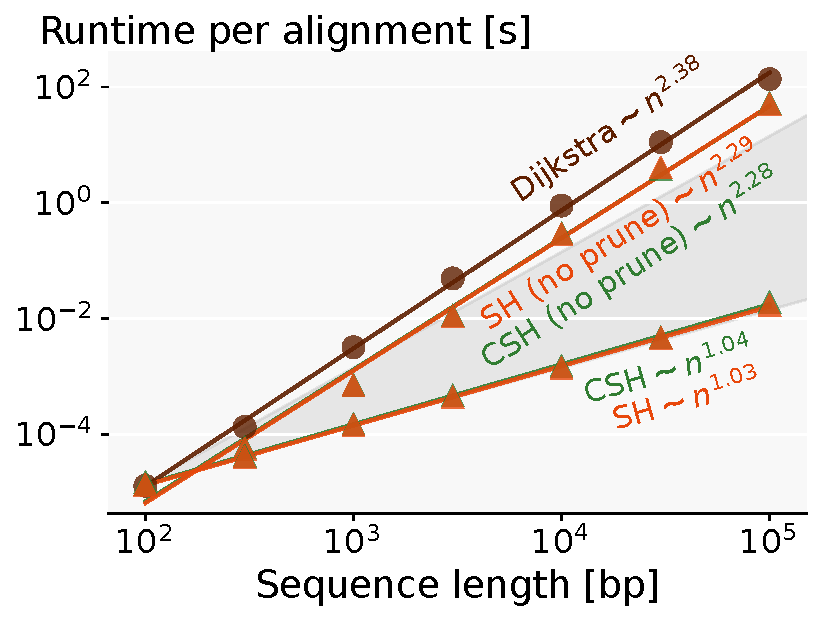
\includegraphics[width=0.45\linewidth]{imgs/fig5/scaling_n_labels.pdf}\label{GLOBALfig:scaling_n}}
  %\hfill
  \subfloat[The effect of chaining and inexact matching on the runtime scaling
  with $e$ ($n{=}10^4$, $k{=}9$, averaged over $100$ alignments).]
  {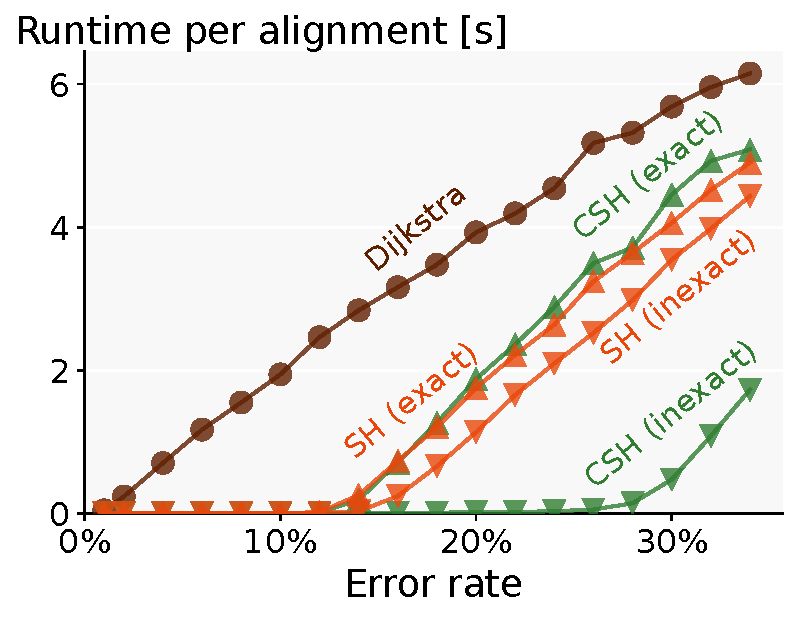
\includegraphics[width=0.45\linewidth]{imgs/fig5/scaling_e_labels.pdf}\label{GLOBALfig:scaling_e}}

  \caption[The effects of pruning, inexact matching, and chaining on runtime
   scaling with length and error rate]{The effects of seed heuristic
   optimizations on runtime scaling (\textbf{synthetic data}).}
  \label{GLOBALfig:scaling}
\end{figure}
